\documentclass{beamer}
\usetheme{Madrid}
\setbeamertemplate{frametitle continuation}{}
\usepackage[T1]{fontenc}
\usepackage{lmodern}
\usepackage{booktabs}
\usepackage{graphicx}
\usepackage{tikz}
\usepackage{listings}
\usetikzlibrary{positioning, arrows.meta, backgrounds}
\usepackage{xspace}
\newcommand{\eg}{e.g.\@\xspace}
\newcommand{\ie}{i.e.\@\xspace}
\newcommand{\etal}{\textit{et al.}\@\xspace}

% \AtBeginSection[]
% {
%   \begin{frame}
%     \frametitle{Table of Contents}
%     \tableofcontents[currentsection]
%   \end{frame}
% }

\title[Short Title]{Long Title}

\author[]{Tran Canh Anh Tuan \and Le Dat Phuc An \\ \and Vong Chi Van \and Pham Nguyen Minh Quan}

\institute[]{
University of Science, VNU-HCM, Viet Nam\\
{\tt\small \{vcvan2424,pnmquan2414\}@apcs.fitus.edu.vn}}
\date{}

\begin{document}

\frame{\titlepage}

\begin{frame}{Table of Contents}
	\tableofcontents
\end{frame}

\section{Introduction}

\begin{frame}{Frame Title}
\end{frame}

% --- Slide 2: Table Summary ---
\begin{frame}{Database Implementation}
    \textbf{Logical Schema implemented in SQL Server via T-SQL DDL}
    \vspace{0.3cm}
    
    \begin{table}
        \centering
        \resizebox{\textwidth}{!}{
            \begin{tabular}{ll}
                \toprule
                \textbf{Table} & \textbf{Purpose} \\
                \midrule
                \textbf{USERS} & Role-based access (students, lecturers, TAs, staff, admins, managers) \\
                \textbf{SPACES} & Campus spaces, types, capacities, and availability statuses \\
                \textbf{FACILITY} & Equipment installed in each space (projectors, computers, etc.) \\
                \textbf{BOOKING\_REQUEST} & Time range, purpose, participant count, and lifecycle status \\
                \textbf{BOOKING\_APPROVAL} & Approval/rejection decisions (at most one per request) \\
                \textbf{USAGE\_SESSION} & Check-in/check-out data for approved bookings \\
                \textbf{MAINTENANCE\_RECORD} & Tracks maintenance issues from report to resolution \\
                \bottomrule
            \end{tabular}
        }
    \end{table}
\end{frame}

% --- Slide 3: Constraints ---
\begin{frame}{Database Constraints}
    \begin{itemize}
        \item \textbf{Primary Keys:} Single-attribute PKs for all 7 tables ensuring 2NF compliance.
        \vspace{0.2cm}
        \item \textbf{Foreign Keys:} 11 FKs implementing all ERD relationships.
        \vspace{0.2cm}
        \item \textbf{CHECK Constraints:} Enforcing strict domain integrity:
        \begin{itemize}
            \item Valid time ranges (\texttt{end\_time > start\_time})
            \item Positive integers for \texttt{capacity} and \texttt{participants}
            \item Strict string mappings for \texttt{role}, \texttt{status}, and \texttt{space\_type}
        \end{itemize}
    \end{itemize}
\end{frame}
\begin{frame}{Database Constraints: UNIQUE}
    \textbf{Four UNIQUE constraints enforce candidate keys and 1:0..1 cardinalities:}
    \vspace{0.3cm}
    
    \begin{itemize}
        \item \textbf{\texttt{USERS.email}}
        \begin{itemize}
            \item Enforces a Candidate Key to prevent duplicate account registrations.
        \end{itemize}
        \vspace{0.2cm}
        \item \textbf{\texttt{SPACES(building, room\_number)}}
        \begin{itemize}
            \item Enforces a Composite Candidate Key to prevent creating the same room twice in one building.
        \end{itemize}
        \vspace{0.2cm}
        \item \textbf{\texttt{BOOKING\_APPROVAL.booking\_id}}
        \begin{itemize}
            \item Enforces 1:0..1 cardinality. Prevents a single booking from having multiple conflicting approval/rejection records.
        \end{itemize}
        \vspace{0.2cm}
        \item \textbf{\texttt{USAGE\_SESSION.booking\_id}}
        \begin{itemize}
            \item Enforces 1:0..1 cardinality. Prevents duplicate active sessions (double check-ins) for the exact same booking.
        \end{itemize}
    \end{itemize}
\end{frame}
% --- Slide 4: Business Rules ---
\begin{frame}{Advanced Business Rules}
    \textit{The following rules involve cross-table validation and require triggers or application logic:}
    \vspace{0.5cm}
    
    \begin{enumerate}
        \item \textbf{Overlapping Bookings:}\\ 
        Preventing approved bookings on the same space with overlapping time ranges.
        \vspace{0.3cm}
        \item \textbf{Space Availability Check:}\\ 
        Verifying a space is not \texttt{under\_maintenance}, \texttt{temporarily\_closed}, or \texttt{retired} before allowing a booking.
        \vspace{0.3cm}
        \item \textbf{Rejection Enforcement:}\\ 
        Ensuring that any rejected booking contains a non-NULL \texttt{rejection\_reason}.
    \end{enumerate}
\end{frame}

% --- Slide 5: Sample Data & Test Coverage (Part 1) ---
\begin{frame}{Sample Data \& Test Coverage }
    \textbf{Comprehensive dataset covering the full range of business scenarios.}
    \vspace{0.3cm}
    
    \begin{itemize}
        \item \textbf{Booking statuses:} Covered all seven statuses: Pending, Approved, Rejected, Cancelled, Checked In, Completed, and No-show.
        \vspace{0.2cm}
        \item \textbf{Space statuses:} Covered Available, Under Maintenance, Temporarily Closed, Retired, and In Use scenarios.
        \vspace{0.2cm}
        \item \textbf{User roles:} Covered Student, Lecturer, Teaching Assistant, Facility Staff, Department Administrator, and Facility Manager.
    \end{itemize}
\end{frame}

% --- Slide 6: Sample Data & Test Coverage (Part 2) ---
\begin{frame}{Sample Data \& Test Coverage }
    \begin{itemize}
        \item \textbf{Maintenance statuses:} Covered Pending, In Progress, Completed, and Cancelled.
        \vspace{0.2cm}
        \item \textbf{Account statuses:} Covered Active, Inactive, and Suspended.
        \vspace{0.2cm}
        \item \textbf{Optional relationship cases:} Included bookings without approval and bookings without usage sessions.
        \vspace{0.2cm}
        \item \textbf{Edge cases:}    
         \begin{itemize}
            \item No-show bookings with prior approval but no session.
            \item Ongoing sessions with NULL \texttt{actual\_end\_time}.
            \item Rejected bookings with recorded reasons.
            \item Maintenance on retired spaces.
        \end{itemize}
    \end{itemize}
\end{frame}

% --- Slide 6: Query Design ---
\begin{frame}{Query Design Summary}
    \textbf{24 queries addressing operational, analytical, and reporting needs.}
    \vspace{0.3cm}
    
    \begin{table}
        \centering
        \resizebox{\textwidth}{!}{
            \begin{tabular}{lll}
                \toprule
                \textbf{\#} & \textbf{Business Question} & \textbf{Target User} \\
                \midrule
                Q18 & Which spaces are available to book right now? & Students/Staff \\
                Q04 & Which booking requests were rejected and why? & Facility Mgr/Admin \\
                Q09 & Have any bookings been approved by unauthorized users? & System Admin \\
                Q05 & Which spaces are used most frequently? & Facility Mgr \\
                Q16 & What is the no-show rate for each user? & Facility Mgr/Admin \\
                Q20 & Which maintenance issues are open $> 7$ days? & Facility Mgr \\
                Q21 & Which users history overstay beyond their end time? & Facility Mgr \\
                \bottomrule
            \end{tabular}
        }
    \end{table}
\end{frame}

% % --- Slide 7: Query Highlight 1 (Fragile frame for code) ---
% \begin{frame}[fragile]{Query Highlight: No-Show Rate (Q16)}
%     \textit{Demonstrates advanced aggregation (\texttt{COUNT}, conditional \texttt{SUM}, \texttt{CAST}).}
    
%     \begin{lstlisting}
% SELECT
%     u.user_id,
%     u.full_name,
%     COUNT(br.booking_id) AS total_bookings,
%     SUM(CASE WHEN br.status = 'no_show' THEN 1 ELSE 0 END) AS no_show_count,
%     CAST(
%         100.0 * SUM(CASE WHEN br.status = 'no_show' THEN 1 ELSE 0 END)
%         / NULLIF(COUNT(br.booking_id), 0)
%         AS DECIMAL(5,2)
%     ) AS no_show_rate_pct
% FROM USERS u
% JOIN BOOKING_REQUEST br ON u.user_id = br.user_id
% GROUP BY u.user_id, u.full_name
% HAVING COUNT(br.booking_id) > 0
% ORDER BY no_show_rate_pct DESC;
%     \end{lstlisting}
% \end{frame}

% % --- Slide 8: Query Highlight 2 (Fragile frame for code) ---
% \begin{frame}[fragile]{Query Highlight: Overdue Maintenance (Q20)}
%     \textit{Demonstrates cross-table logic, \texttt{LEFT JOIN}s, and temporal functions (\texttt{DATEDIFF}).}
    
%     \begin{lstlisting}
% SELECT
%     m.maintenance_id,
%     s.space_name,
%     m.problem_description,
%     u_rep.full_name AS reporter_name,
%     u_asgn.full_name AS assigned_staff_name,
%     DATEDIFF(DAY, m.start_time, GETDATE()) AS days_open
% FROM MAINTENANCE_RECORD m
% JOIN SPACES s ON m.space_code = s.space_code
% JOIN USERS u_rep ON m.reporter_user_id = u_rep.user_id
% LEFT JOIN USERS u_asgn ON m.assigned_staff_user_id = u_asgn.user_id
% WHERE m.status IN ('open', 'in_progress')
%   AND DATEDIFF(DAY, m.start_time, GETDATE()) > 7;
%     \end{lstlisting}
% \end{frame}
% ====================================================================
% Section: AI Agent Improvement Process
% ====================================================================
\section{AI Agent Improvement Process}

% --- Slide: Architecture Overview ---
\begin{frame}{Agent Architecture}
    \textbf{A two-layer knowledge system guides the LLM throughout the project.}
    \vspace{0.3cm}

    \begin{columns}[T]
        \column{0.48\textwidth}
        \textbf{Agent (Global Knowledge)}
        \begin{itemize}
            \item Source-of-truth schema
            \item Non-negotiable business rules
            \item Global consistency rules
            \item Verification behavior
        \end{itemize}

        \column{0.48\textwidth}
        \textbf{Skills (Section-Specific)}
        \begin{itemize}
            \item Methodology \& checklists
            \item Verification procedures
            \item Common mistakes
            \item Anti-hallucination rules
        \end{itemize}
    \end{columns}

    \vspace{0.4cm}
    \centering
    \small\textit{7 sections $\times$ 3 rounds each = 21 experiment iterations}
\end{frame}

% --- Slide: Iterative Workflow ---
\begin{frame}{Iterative Improvement Workflow}
    \textbf{Each section undergoes a 3-round experiment cycle:}
    \vspace{0.3cm}

    \begin{center}
        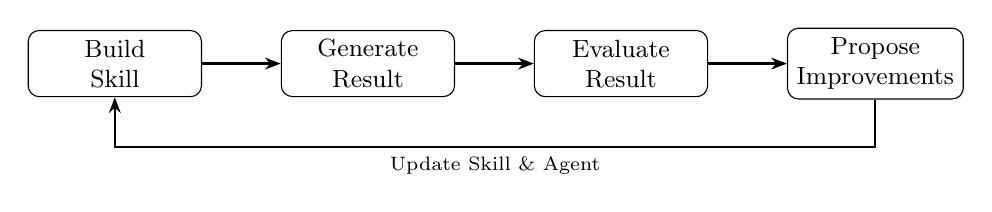
\begin{tikzpicture}[
            node distance=0.4cm and 1.0cm,
            box/.style={draw, rounded corners, minimum width=2.2cm, minimum height=0.7cm, align=center, font=\small},
            arr/.style={-{Stealth[length=2mm]}, thick}
        ]
            % Row 1: Main flow
            \node[box] (skill) {Build\\Skill};
            \node[box, right=of skill] (gen) {Generate\\Result};
            \node[box, right=of gen] (eval) {Evaluate\\Result};
            \node[box, right=of eval] (improve) {Propose\\Improvements};

            \draw[arr] (skill) -- (gen);
            \draw[arr] (gen) -- (eval);
            \draw[arr] (eval) -- (improve);

            % Feedback loop
            \draw[arr] (improve.south) -- ++(0,-0.6) -| (skill.south)
                node[pos=0.25, below, font=\scriptsize] {Update Skill \& Agent};
        \end{tikzpicture}
    \end{center}

    \vspace{0.2cm}
    \begin{itemize}
        \item \textbf{Round 1:} Baseline --- initial skill generates the first benchmark.
        \item \textbf{Round 2:} Lessons from Round 1 refine the skill before regenerating.
        \item \textbf{Round 3:} Accumulated lessons produce the final benchmark.
    \end{itemize}
\end{frame}

% --- Slide: Evaluation & Learning ---
\begin{frame}{Evaluation \& Learning}
    \begin{columns}[T]
        \column{0.48\textwidth}
        \textbf{Evaluation Dimensions}
        \begin{itemize}
            \item Requirement coverage
            \item Correctness
            \item Naming consistency
            \item Hallucination risk
            \item Documentation quality
            \item Maintainability
        \end{itemize}

        \column{0.48\textwidth}
        \textbf{Learning Mechanism}
        \begin{itemize}
            \item Each round produces an \texttt{ImproveXX} document
            \item Records issues, root causes, and proposed fixes
            \item Knowledge is \textbf{cumulative} --- never discarded
            \item Lessons are classified: Agent-level vs.\ Skill-level
        \end{itemize}
    \end{columns}

    \vspace{0.3cm}
    \centering
    \small\textit{Human approval is required at every step --- the agent proposes, never applies.}
\end{frame}

% --- Slide: Key Design Principles ---
\begin{frame}{Key Design Principles}
    \begin{enumerate}
        \item \textbf{Human-in-the-Loop:} The agent proposes changes; humans approve before any modification is applied.
        \vspace{0.2cm}
        \item \textbf{Separation of Concerns:} Dedicated workers for skill building, result generation, evaluation, and improvement --- no worker exceeds its role.
        \vspace{0.2cm}
        \item \textbf{Cumulative Knowledge:} Skills and improvement documents grow over rounds; previous lessons are preserved and refined.
        \vspace{0.2cm}
        \item \textbf{Anti-Hallucination:} Workers operate only on explicitly injected files; no repository exploration or hidden context is allowed.
    \end{enumerate}
\end{frame}

% \begin{frame}[allowframebreaks]{References}
% 	\bibliographystyle{plain} % or unsrt, alpha, abbrv
% 	\bibliography{main}
% \end{frame}

\end{document}
